\chapter{This is the first real chapter}


\lipsum[1-2]


The well known Pythagorean theorem \(x^2 + y^2 = z^2\) was 
proved to be invalid for other exponents. 
Meaning the next equation has no integer solutions:

\begin{equation}
	x^n + y^n = z
	.
\end{equation}
\lipsum[3-4]

\begin{figure}[h]
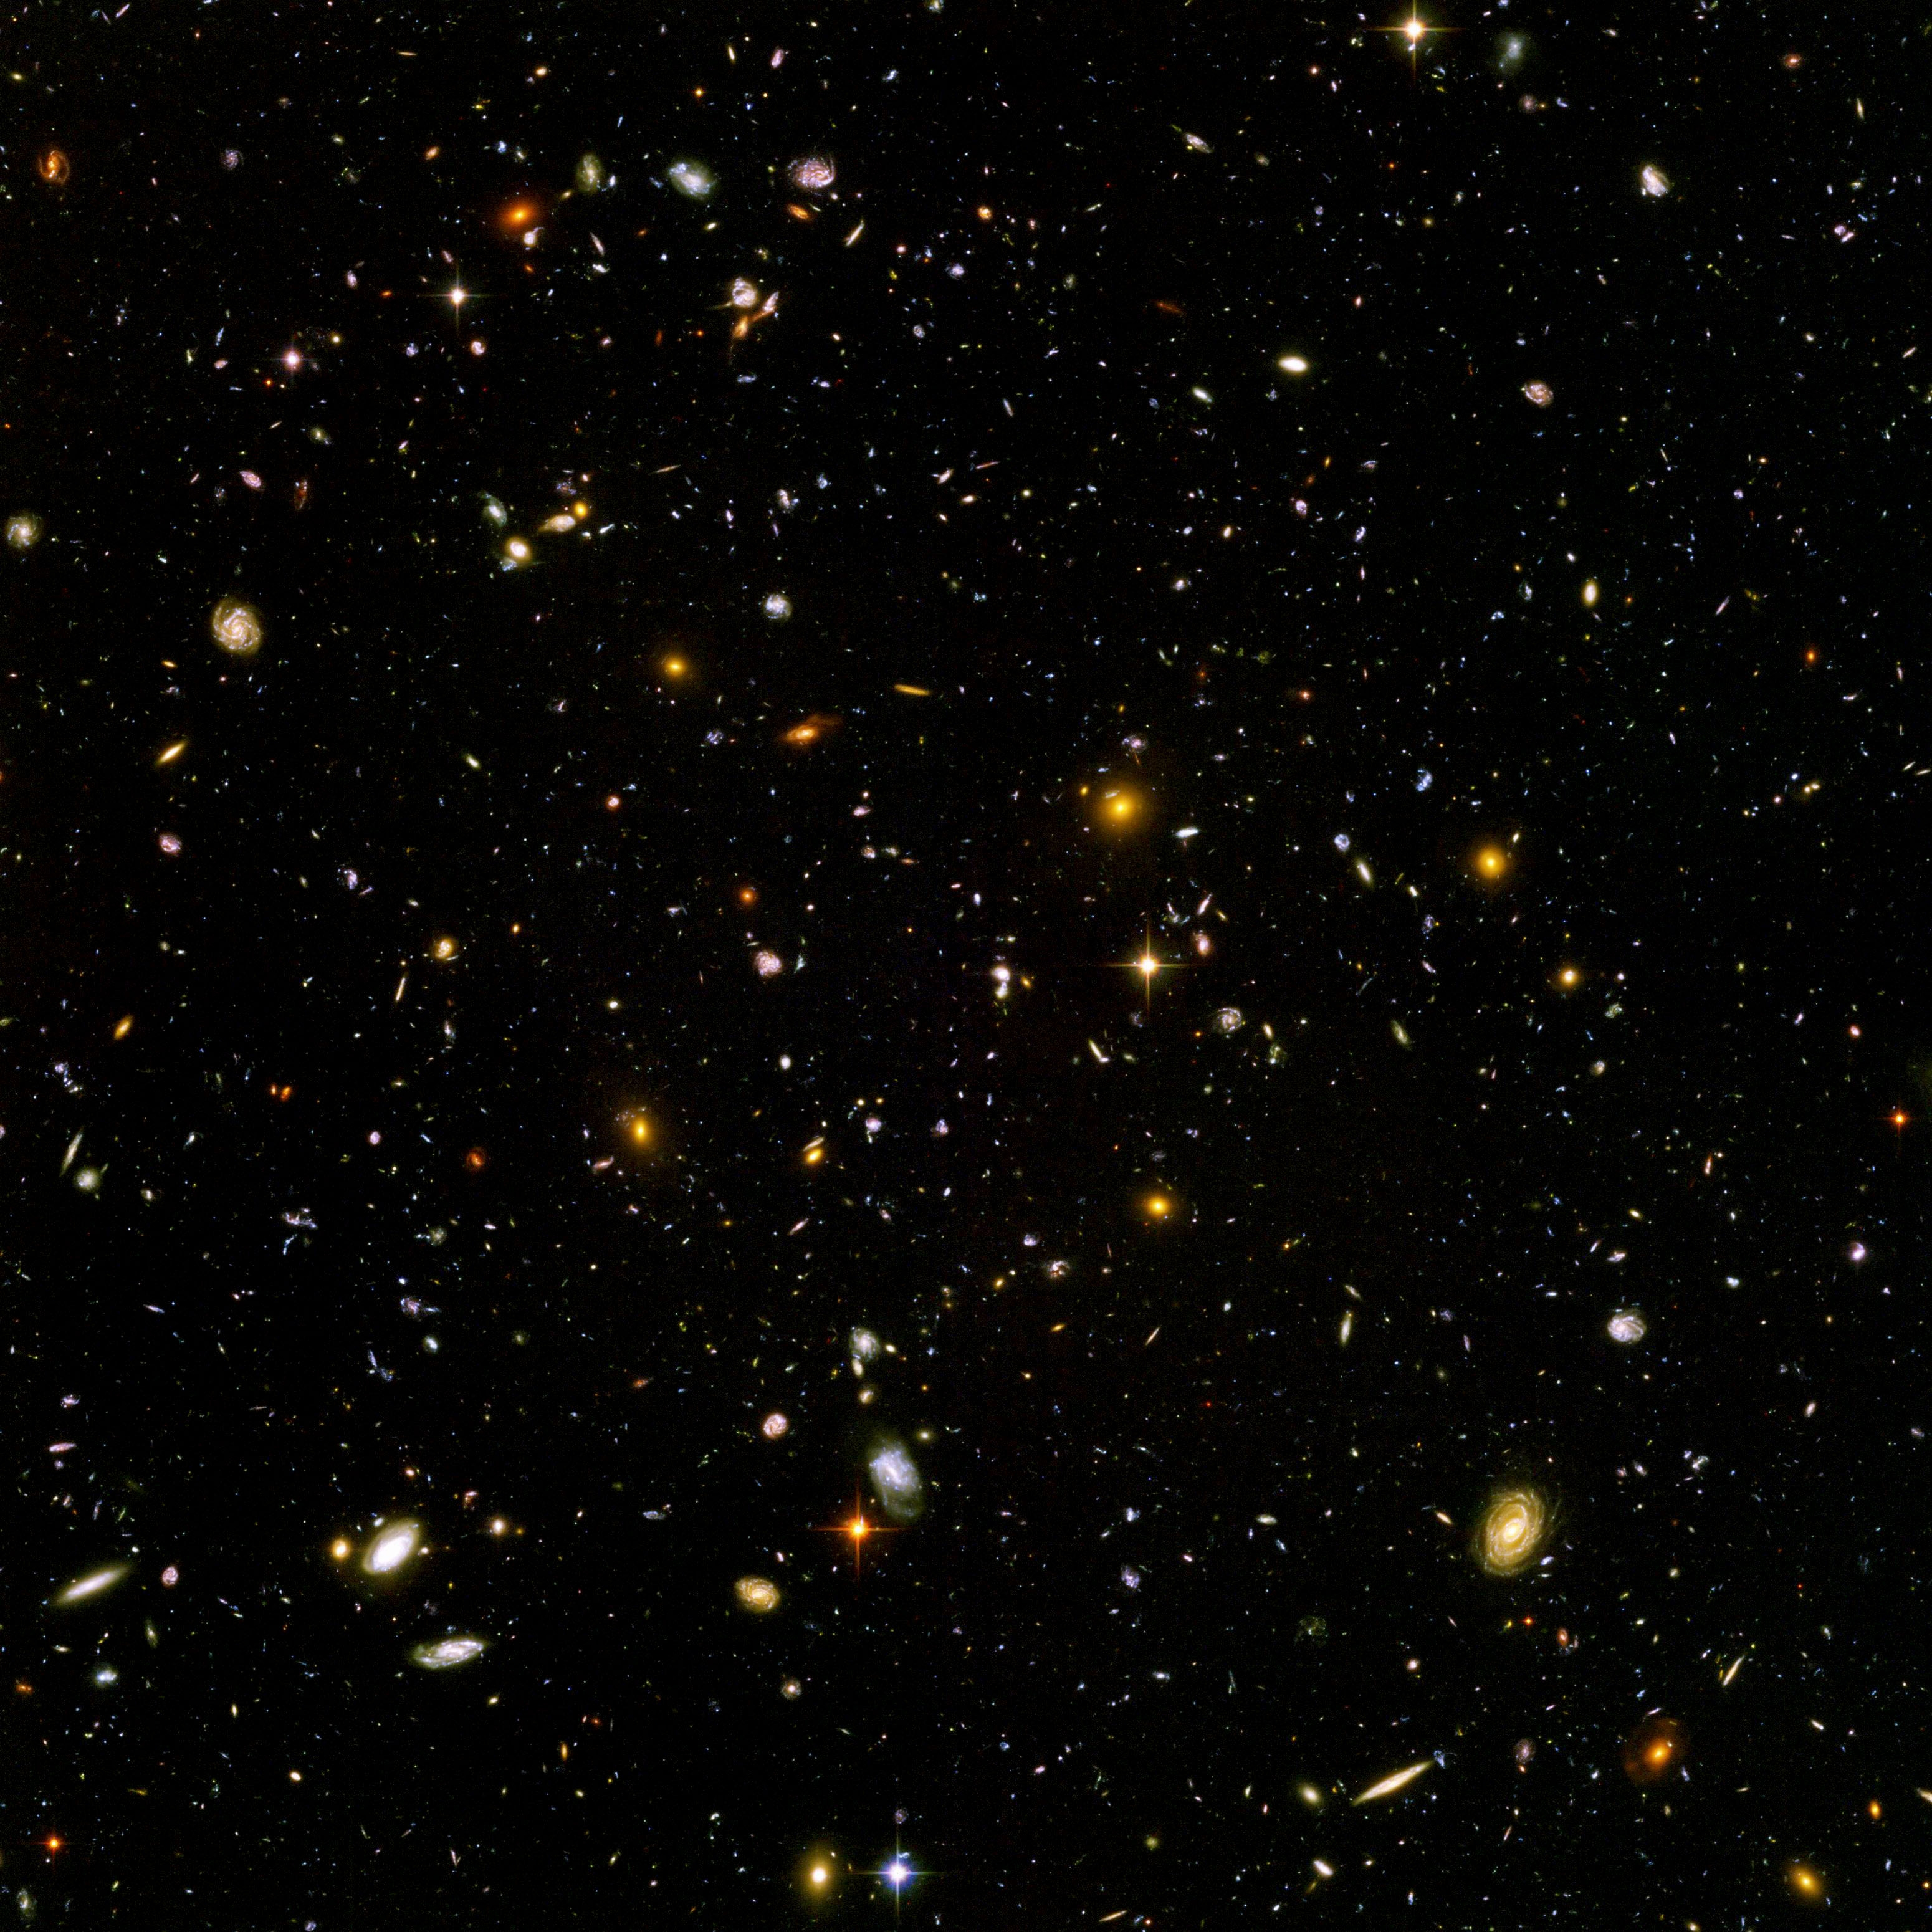
\includegraphics[width=\textwidth]{./chapters/chapter1/figures/Hubble_ultra_deep_field.jpg}
\caption{WikiPedia: ``The Hubble Ultra Deep Field, is an image of a small region of space in the constellation Fornax, composited from Hubble Space Telescope data accumulated over a period from September 3, 2003 through January 16, 2004. The patch of sky in which the galaxies reside was chosen because it had a low density of bright stars in the near-field.'' Copyright: NASA and the European Space Agency -- \url{http://hubblesite.org/newscenter/archive/releases/2004/07/image/a/warn/}.}
\end{figure}
